%!TEX program=xelatex

\documentclass[11pt]{ctexart}  
\usepackage[top=2cm, bottom=2cm, left=2cm, right=2cm]{geometry}  
\usepackage{algorithm}  
\usepackage{algorithmicx}  
\usepackage{algpseudocode}  
\usepackage{amsmath}  
\usepackage{graphicx}
\usepackage{amsmath}
\usepackage{amssymb}
\usepackage{enumerate}
\usepackage{booktabs}
\usepackage{fontspec}
\usepackage{listings}
\usepackage{xcolor}

\newfontfamily\monaco{Monaco}
\definecolor{mygreen}{rgb}{0,0.6,0}
\definecolor{mygray}{rgb}{0.5,0.5,0.5}
\definecolor{mymauve}{rgb}{0.58,0,0.82}
\lstset{ %
backgroundcolor=\color{white},      % choose the background color
basicstyle=\footnotesize\ttfamily,  % size of fonts used for the code
columns=fullflexible,
tabsize=4,
breaklines=true,               % automatic line breaking only at whitespace
captionpos=b,                  % sets the caption-position to bottom
commentstyle=\color{mygreen},  % comment style
escapeinside=``,        % if you want to add LaTeX within your code
keywordstyle=\color{blue},     % keyword style
stringstyle=\color{mymauve}\ttfamily,  % string literal style
frame=single,
rulesepcolor=\color{red!20!green!20!blue!20},
language=python,
}

\floatname{algorithm}{算法}
\renewcommand{\algorithmicrequire}{\textbf{输入:}}  
\renewcommand{\algorithmicensure}{\textbf{输出:}} 

\title{密码学实验报告10}
\author{张天辰 17377321}

\makeatletter
\newenvironment{breakablealgorithm}
  {% \begin{breakablealgorithm}
   \begin{center}
     \refstepcounter{algorithm}% New algorithm
     \hrule height.8pt depth0pt \kern2pt% \@fs@pre for \@fs@ruled
     \renewcommand{\caption}[2][\relax]{% Make a new \caption
       {\raggedright\textbf{\ALG@name~\thealgorithm} ##2\par}%
       \ifx\relax##1\relax % #1 is \relax
         \addcontentsline{loa}{algorithm}{\protect\numberline{\thealgorithm}##2}%
       \else % #1 is not \relax
         \addcontentsline{loa}{algorithm}{\protect\numberline{\thealgorithm}##1}%
       \fi
       \kern2pt\hrule\kern2pt
     }
  }{% \end{breakablealgorithm}
     \kern2pt\hrule\relax% \@fs@post for \@fs@ruled
   \end{center}
  }
\makeatother

\begin{document}
\maketitle{}
\section{SM2数字签名算法} % (fold)
\subsection{算法原理} % (fold)
SM2算法利用椭圆曲线构造数字签名。以下流程不考虑边界情况。首先根据椭圆曲线参数、用户的公钥$P_A$和用户的个人身份构造身份信息$Z_A$。将$Z_A$和消息$M$组合到一起,再经过Hash函数得到$e$。此后产生随机数$k$,并计算$(x_1, y_1) = kG$。令$r = (e + x_1) \mod n$,$s = \frac{k - rd_A}{1 + d_A} \mod n$。签名即为$(r, s)$。

签名的验证方法如下。由生成过程可知,重要的在于恢复$k$。首先用与生成签名相同的方法可以得到$e$,此后令$t = r + s$,则有:
$$t = r + s = \frac{k - rd_A}{1 + d_A} + r = \frac{k + r}{1 + d_A}$$
$$s + td_A = \frac{kd_A + rd_A + k - rd_A}{1 + d_A} = k$$
因此可以如上恢复出$k$。从而可以恢复$x_1$,并计算$R = (e + x_1) \mod n$与收到的$r$进行验证。如果相等则验证成功。
% subsection 算法原理 (end)
\subsection{算法实现} % (fold)
关于椭圆曲线上的运算以及类型转换等算法可以直接复用先前实现SM2公钥算法时的代码。
\begin{enumerate}
    \item 签名生成算法
    \begin{lstlisting}[language={python},
    numbers=left,
    numberstyle=\tiny\monaco,
    basicstyle=\small\monaco]
    def sign(message):
        za = sm3(entl || id || a || b || g.x || g.y || public.x || public.y)
        m1 = za || message
        e = sm3(m1)
        while True:
            k = randint(1, n - 1)
            temp = g.multi(k)
            r = (e + temp.x) mod n
            if r == 0 or r + k == n:
                continue
            s = (reverse(1 + private, n) * (k - r * private)) mod n
            if s != 0:
                break
        return (r, s)
    \end{lstlisting}
    \item 签名验证算法
    \begin{lstlisting}[language={python},
    numbers=left,
    numberstyle=\tiny\monaco,
    basicstyle=\small\monaco]
    def authenticate(message, signature):
        r = signature[0]
        s = signature[1]
        if r < 1 or r >= n or s < 1 or s >= n:
            return False
        za = sm3(entl || id || a || b || g.x || g.y || public.x || public.y)
        m1 = za || message
        e = sm3(m1)
        t = (r + s) mod n
        if t == 0:
            return False
        temp = g.multi(s) + public.multi(t)
        R = (e + temp.x) mod n
        if R == r:
            return True
        else:
            return False
    \end{lstlisting}
\end{enumerate}
% subsection 算法实现 (end)
\subsection{算法测试} % (fold)
这里采用SM2标准中的测试数据进行检验。用户ID为ALICE123@YAHOO.COM,发送的消息为message digest,椭圆曲线参数、公私钥等参数比较复杂,略去。
对这组数据,标准的结果为:

$r = $ 0x40F1EC59F793D9F49E09DCEF49130D4194F79FB1EED2CAA55BACDB49C4E755D1

$s = $ 0x6FC6DAC32C5D5CF10C77DFB20F7C2EB667A457872FB09EC56327A67EC7DEEBE7

如图\ref{img_sign}所示,使用上述内容进行数字签名,得到的结果与标准相同。标准的结果按照十六进制数的形式给出,但根据标准的算法流程,这里的签名应该是字节串,因此本实现按照字节串输出,不难验证两者的相同性。此后,使用上述签名进行验证(图\ref{img_sign}代码第88行),得到了认证通过的结果;使用另外的签名进行认证(图\ref{img_sign}中代码第89行),则认证不通过。

\begin{figure}[htbp]
\centering
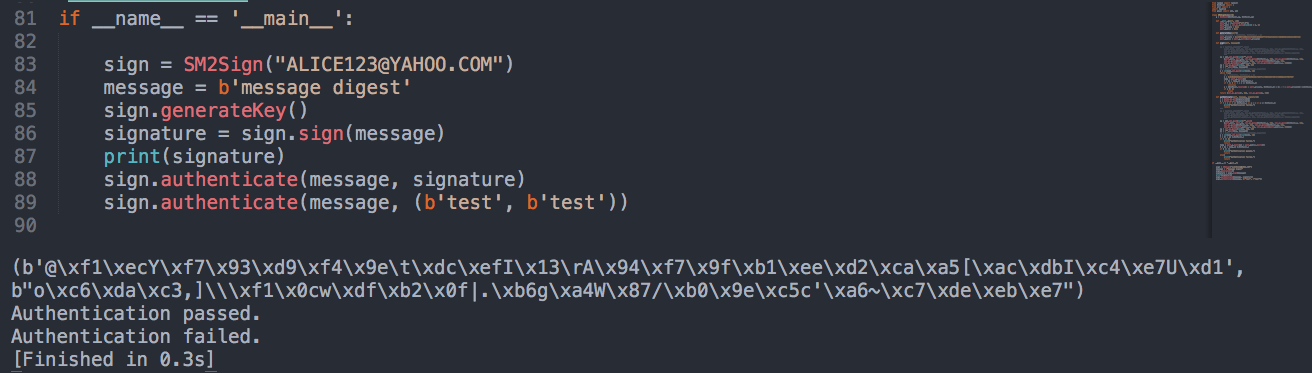
\includegraphics[width=13.12cm, height=3.73cm]{sign.png}
\caption{SM2数字签名算法测试}
\label{img_sign}
\end{figure}
% subsection 算法测试 (end)
% section sm2数字签名算法 (end)
\section{感想} % (fold)
这次实验相对而言比较容易。我认为在初级、中级、高级要求中选择一个进行实现是很合理的制度,因为对于本次实验而言,不同的要求只是实现的数字签名算法不太一样而已,而不管实现哪种,都是按照标准一步一步实现。只要实现了一种,就能加深对数字签名的理解。
% section 感想 (end)
\end{document}